\documentclass[11pt,a4paper]{article}

% ── Packages ──────────────────────────────────────────────
\usepackage[margin=1in]{geometry}
\usepackage{enumitem}
\usepackage{booktabs}
\usepackage{longtable}
\usepackage{xcolor}
\usepackage{hyperref}
\usepackage{tikz}
\usetikzlibrary{arrows.meta, positioning, shapes.geometric, calc}
\usepackage{amsmath,amssymb}
\usepackage{tcolorbox}
\usepackage{tabularx}
\usepackage{fancyhdr}
\usepackage{titlesec}
\usepackage{parskip}

% ── Colors ────────────────────────────────────────────────
\definecolor{critical}{RGB}{180,40,40}
\definecolor{deepening}{RGB}{40,100,160}
\definecolor{success}{RGB}{30,120,60}
\definecolor{warn}{RGB}{200,140,20}
\definecolor{lightgray}{RGB}{245,245,245}

% ── Environments ──────────────────────────────────────────
\newtcolorbox{successbox}[1][]{
  colback=success!5, colframe=success!70!black,
  fonttitle=\bfseries, title=Success Criteria, #1
}
\newtcolorbox{deepbox}[1][]{
  colback=deepening!5, colframe=deepening!70!black,
  fonttitle=\bfseries, title=Deepenings (if time permits), #1
}
\newtcolorbox{warnbox}[1][]{
  colback=warn!8, colframe=warn!80!black,
  fonttitle=\bfseries, title=Kill / Pivot Criteria, #1
}
\newtcolorbox{depbox}[1][]{
  colback=lightgray, colframe=black!40,
  fonttitle=\bfseries, title=Dependencies, #1
}

% ── Header / Footer ──────────────────────────────────────
\pagestyle{fancy}
\fancyhf{}
\lhead{\small 15.458 Project F --- Action Plan}
\rhead{\small Spring 2026}
\cfoot{\thepage}

% ── Section formatting ────────────────────────────────────
\titleformat{\section}{\Large\bfseries\color{critical!80!black}}{Phase \thesection:}{0.5em}{}
\titleformat{\subsection}{\large\bfseries}{Task \thesubsection:}{0.5em}{}

\begin{document}

% ══════════════════════════════════════════════════════════
% TITLE
% ══════════════════════════════════════════════════════════
\begin{center}
  {\LARGE\bfseries Exhaustive Action Plan}\\[6pt]
  {\Large Stress-Testing High-Frequency Market Makers\\
  with Diffusion-Generated Counterfactual LOBs}\\[10pt]
  {\large 15.458 Financial Data Science and Computing --- Spring 2026}\\[4pt]
  {\normalsize Arturo Favara \quad Nick Bernardini \quad Maxime Vallot}\\[4pt]
  {\small Document date: April 18, 2026}
\end{center}

\vspace{0.3cm}
\hrule height 0.8pt
\vspace{0.5cm}

% ══════════════════════════════════════════════════════════
% 0. PREAMBLE
% ══════════════════════════════════════════════════════════
\section*{How to Read This Document}

This action plan is organized into \textbf{seven sequential phases}, each decomposed into atomic tasks.
Every task specifies:

\begin{enumerate}[label=(\roman*)]
  \item \textbf{What} needs to be done, with enough detail to start immediately.
  \item \textbf{Success criteria}: concrete, measurable conditions that mark a task as complete.
  \item \textbf{Dependencies}: which earlier tasks must be finished first.
  \item \textbf{Deepenings}: optional extensions to pursue if the core is done early.
  \item \textbf{Kill / pivot criteria}: conditions under which the task's scope should be reduced or the project should change direction.
  \item \textbf{Owner}: which team role is primarily responsible (Data Lead, ML Lead, Validation+MM Lead, Analysis+Writing Lead).
\end{enumerate}

The phases are strictly ordered at the macro level (you cannot train a generator before the data pipeline exists), but many tasks within a phase can proceed in parallel across team members.
A dependency graph is provided at the end of the document.

\vspace{0.4cm}
\hrule height 0.4pt

% ══════════════════════════════════════════════════════════
%  PHASE 0: INFRASTRUCTURE
% ══════════════════════════════════════════════════════════
\setcounter{section}{-1}
\section{Infrastructure and Environment Setup}

\textit{Goal: Every team member can run code, access data, and track experiments from day one.}

\subsection{Repository and Version Control}

\textbf{What.}
Create a single Git repository (GitHub or MIT GitLab).
Establish the following directory layout:

\begin{verbatim}
  /data/raw/          # Raw TAQ / LOBSTER downloads (gitignored)
  /data/processed/    # Parquet event tapes, regime features
  /src/data/          # Data pipeline code
  /src/generator/     # DDPM / DDIM training and sampling
  /src/agents/        # MM agent implementations
  /src/evaluation/    # Backtest runner, metrics, ranking test
  /configs/           # Hydra YAML configs
  /notebooks/         # Exploratory notebooks (numbered)
  /reports/           # LaTeX source for final report
  /checkpoints/       # Model checkpoints (gitignored, symlinked)
  /results/           # Output CSVs, figures
\end{verbatim}

Set up a \texttt{.gitignore} for data, checkpoints, and \texttt{wandb/} logs.
Write a \texttt{README.md} with a one-command setup script.

Add a \texttt{Makefile} (or \texttt{justfile}) with targets: \texttt{make data}, \texttt{make train}, \texttt{make sample}, \texttt{make backtest}, \texttt{make report}.

\begin{successbox}
  \begin{itemize}[nosep]
    \item Every team member can clone, install, and run a trivial smoke test within 15 minutes.
    \item Branch protection on \texttt{main}; all merges via PR.
    \item Reproducibility: every experiment tied to a git commit hash.
  \end{itemize}
\end{successbox}

\textbf{Owner:} Everyone (day-one session). \quad \textbf{Effort:} 2--3 hours.

\subsection{Python Environment and Dependencies}

\textbf{What.}
Pin a Python version ($\geq 3.11$). Create a \texttt{pyproject.toml} or \texttt{environment.yml} with all dependencies:

\begin{itemize}[nosep]
  \item \textbf{Core:} \texttt{torch $\geq$ 2.2}, \texttt{pytorch-lightning}, \texttt{hydra-core}, \texttt{wandb}.
  \item \textbf{Diffusion:} \texttt{diffusers}, \texttt{einops}; clone \texttt{DeepMarket} repo locally.
  \item \textbf{Data:} \texttt{pandas}, \texttt{polars}, \texttt{pyarrow}, \texttt{numpy}, \texttt{scipy}, \texttt{statsmodels}, \texttt{wrds}.
  \item \textbf{Evaluation:} \texttt{scikit-learn}, \texttt{matplotlib}, \texttt{seaborn}.
  \item \textbf{Optional:} \texttt{abides-core}, \texttt{abides-markets} (only if interactive sim is attempted), \texttt{lob-bench} (if pip-installable; otherwise vendor the code).
\end{itemize}

Verify GPU access: run a 10-step dummy DDPM forward--reverse on a random tensor.

\begin{successbox}
  \begin{itemize}[nosep]
    \item \texttt{pip install -e .} or \texttt{conda env create} succeeds on all team machines and on the cluster.
    \item \texttt{import torch; torch.cuda.is\_available()} returns \texttt{True} on at least one GPU node.
    \item DeepMarket/TRADES can be imported without error.
  \end{itemize}
\end{successbox}

\textbf{Owner:} ML Lead + Data Lead. \quad \textbf{Effort:} half-day.

\subsection{Compute Access and Experiment Tracking}

\textbf{What.}
\begin{enumerate}[nosep]
  \item Confirm GPU allocation on MIT SuperCloud or OpenMind.  Document the SLURM commands and partition names the team should use.
  \item Set up a shared Weights \& Biases (wandb) project.  Every training run and every backtest logs to wandb with: config hash, git SHA, all hyperparameters, and loss curves.
  \item Set up a shared Google Sheet or Notion board for manual tracking of milestone status.
\end{enumerate}

\begin{successbox}
  \begin{itemize}[nosep]
    \item A dummy SLURM job runs to completion on a GPU node and logs a metric to wandb.
    \item The team can view each other's runs in the wandb dashboard.
  \end{itemize}
\end{successbox}

\textbf{Owner:} ML Lead. \quad \textbf{Effort:} half-day.


% ══════════════════════════════════════════════════════════
%  PHASE 1: DATA PIPELINE
% ══════════════════════════════════════════════════════════
\section{Data Pipeline}

\textit{Goal: Produce clean, validated Parquet event tapes and regime-feature vectors for INTC (primary) and TSLA (stretch), ready for generator training.}

\subsection{Data Acquisition}

\textbf{What.}
\begin{enumerate}[nosep]
  \item Log in to WRDS.  Confirm access to NYSE Daily TAQ tables: \texttt{ctm\_consolidated\_trades}, \texttt{cqm\_consolidated\_quotes}, and \texttt{complete\_nbbo}.
  \item Determine whether Sloan's license includes \textbf{NYSE TAQ PLUS / Integrated Feed} (top-10 depth).  If yes, note the table names.  If no, proceed with LOBSTER as the depth source.
  \item For LOBSTER: request or download message-level data for INTC and TSLA for the required date range.  LOBSTER provides free 1-day samples; a full license may be needed for 60+ training days.
  \item Define date ranges:
    \begin{itemize}[nosep]
      \item \textbf{Training:} 60 trading days (approximately Mar--May 2025).
      \item \textbf{Validation:} 10 trading days (Jun 2025).
      \item \textbf{Holdout:} 20 trading days (Jul--Aug 2025), including at least one CPI/FOMC/earnings day.
    \end{itemize}
  \item Download all raw data.  Record MD5 hashes of every downloaded file in a manifest (\texttt{data/raw/MANIFEST.md5}).
\end{enumerate}

\begin{successbox}
  \begin{itemize}[nosep]
    \item Raw data for INTC (and TSLA if feasible) sits in \texttt{data/raw/} with documented hashes.
    \item A clear written record states whether depth data comes from TAQ PLUS or LOBSTER, with justification.
    \item Holdout window includes $\geq 1$ identifiable stress day (FOMC, CPI, earnings).  This is verified by looking up the macro/earnings calendar.
  \end{itemize}
\end{successbox}

\begin{warnbox}
  If neither TAQ PLUS nor LOBSTER is accessible for the required date range, fall back to \textbf{NBBO-only top-of-book tapes} (the ``reduced paper'' framing).  The generator then models $(p^b, p^a, q^b, q^a, \tau)$ sequences only.  This is still a valid project, just with less depth information.
\end{warnbox}

\textbf{Owner:} Data Lead. \quad \textbf{Effort:} 1--2 days.

\subsection{Data Cleaning and Event-Tape Construction}

\textbf{What.}
Write a deterministic, configurable pipeline (\texttt{src/data/build\_tapes.py}) that:

\begin{enumerate}[nosep]
  \item Filters to the continuous trading session: \textbf{09:45--15:45 ET}, excluding opening and closing auctions.
  \item Removes crossed or locked quotes ($p^b \geq p^a$).
  \item Removes non-firm quote conditions (check \texttt{qu\_cond} flags per TAQ documentation).
  \item Removes corrected or out-of-sequence trades (\texttt{tr\_corr $\neq$ 0}).
  \item Signs trades using Lee--Ready (compare trade price to prevailing midpoint; use tick rule for ties) or Bulk Volume Classification (BVC).  Implement \textit{both} and keep a config toggle.
  \item If using LOBSTER: run Algorithm~1 from the proposal (LOB reconstruction from message-level data).  Sanity-check: bid $<$ ask always, no negative sizes, no crossed books.
  \item If using NBBO-only TAQ: the event tape is the sequence of quote/trade updates with fields $(t, p^b, p^a, q^b, q^a, \text{trade\_price}, \text{trade\_size}, \text{trade\_sign})$.
  \item Compute midprice $m_t = (p^a_t + p^b_t)/2$ and spread $s_t = p^a_t - p^b_t$ at every event.
  \item Output: one Parquet file per (ticker, date) with all fields, sorted by timestamp.
\end{enumerate}

\begin{successbox}
  \begin{itemize}[nosep]
    \item A second team member can run \texttt{python build\_tapes.py --ticker INTC --start 2025-03-01 --end 2025-08-31} and reproduce byte-identical Parquet files (verified by hash).
    \item Zero crossed-book events survive cleaning.
    \item Trade-signing coverage $>$ 95\% (fraction of trades assigned a sign).
    \item Basic sanity statistics printed: events/day, median spread, median inter-event time, fraction of trades vs.\ quote updates.  These are logged and compared against published microstructure benchmarks for INTC.
  \end{itemize}
\end{successbox}

\begin{deepbox}
  \begin{itemize}[nosep]
    \item If LOBSTER depth is available: reconstruct full top-10 depth profiles $L_t(k)$ for $|k| \leq 10$.  Store as a separate depth-Parquet alongside the event tape.
    \item Compare Lee--Ready vs.\ BVC trade signing and document the concordance rate.
    \item Run the pipeline for TSLA in addition to INTC.
  \end{itemize}
\end{deepbox}

\textbf{Owner:} Data Lead. \quad \textbf{Effort:} 3--5 days (the single hardest data task).

\subsection{Regime Feature Engineering}

\textbf{What.}
For every event $i$ at time $t_i$, compute a regime-feature vector $c^{(i)}$:

\begin{center}
\begin{tabular}{llp{7cm}}
\toprule
\textbf{Feature} & \textbf{Window} & \textbf{Definition} \\
\midrule
$c_{\text{vol}}$ & 5 min & Realized volatility $\sigma_t = \sqrt{\sum_{s \in W}(\Delta \log S_s)^2}$, discretized to 3 buckets (low/mid/high) by training-set quantiles. \\
$c_{\text{vpin}}$ & Rolling 50 vol-buckets & VPIN as per Easley--L\'opez de Prado--O'Hara (2012), discretized to 3 buckets. \\
$c_{\text{imb}}$ & Instantaneous & Top-of-book imbalance $I_t = \frac{L_t(-1) - L_t(+1)}{L_t(-1) + L_t(+1)}$, discretized to 3 buckets ($< -0.3$, $[-0.3,0.3]$, $> 0.3$). \\
$c_{\text{tod}}$ & Instantaneous & Time-of-day: morning / midday / afternoon. \\
\bottomrule
\end{tabular}
\end{center}

Implementation steps:
\begin{enumerate}[nosep]
  \item Compute the raw continuous features first.
  \item Determine discretization quantiles on the \textbf{training set only} and freeze them.
  \item Apply those quantile thresholds to validation and holdout sets.
  \item Store the regime vector alongside the event tape in the same Parquet (additional columns).
  \item Write a utility that, given a regime-feature vector, returns the human-readable label: \texttt{base}, \texttt{high\_vol}, \texttt{toxic}, \texttt{thin} (as defined in the proposal's 4-cell summary).
\end{enumerate}

\begin{successbox}
  \begin{itemize}[nosep]
    \item Quantile boundaries are computed, documented, and stored in a JSON config file.
    \item The distribution of regime labels across training days is roughly uniform by construction (since we're using quantiles).
    \item Holdout days are confirmed to include at least one day in each of the stress categories (high\_vol, toxic, or thin).  If not, re-examine the holdout window choice.
    \item VPIN implementation is validated against a known reference (e.g., the original ELP paper's reported VPIN for a similar stock in a similar period, or a cross-check with a second implementation).
  \end{itemize}
\end{successbox}

\begin{deepbox}
  \begin{itemize}[nosep]
    \item Add OFI (order-flow imbalance) as a fifth regime feature, using the sign conventions in Appendix~A of the proposal.
    \item Explore whether finer discretization (5 buckets instead of 3) improves conditional generation quality.
    \item Produce exploratory plots: regime label over time for selected days; scatterplots of $c_{\text{vol}}$ vs.\ $c_{\text{vpin}}$.
  \end{itemize}
\end{deepbox}

\textbf{Owner:} Data Lead. \quad \textbf{Effort:} 2--3 days.

\subsection{Train / Validation / Holdout Splits and Canonical Parquet Files}

\textbf{What.}
\begin{enumerate}[nosep]
  \item Partition the cleaned event-tape Parquets into three directories: \texttt{data/processed/train/}, \texttt{data/processed/val/}, \texttt{data/processed/holdout/}.
  \item Create a \texttt{data/processed/SPLITS.json} listing exact dates in each split.
  \item The holdout directory is \textbf{read-only} after this step.  No code should touch holdout files until Phase~5.
  \item Write a \texttt{DataLoader} / dataset class (\texttt{src/data/lob\_dataset.py}) that:
    \begin{itemize}[nosep]
      \item Loads event tapes for a given split.
      \item Yields windows of $L$ consecutive events (with configurable $L$, default 256 or 512) and their regime conditioning vector $c$.
      \item Applies normalization (zero-mean, unit-variance per feature, computed on training set).
      \item Returns tensors of shape $(L, d)$ where $d = 4 + 2K$ for depth data or $d \approx 5$--7 for top-of-book-only.
    \end{itemize}
\end{enumerate}

\begin{successbox}
  \begin{itemize}[nosep]
    \item \texttt{DataLoader} yields batches without error for at least one full epoch.
    \item Normalization statistics (mean, std per feature) are saved and re-loaded deterministically.
    \item A quick histogram of window lengths confirms no degenerate windows (all-zero, single event, etc.).
  \end{itemize}
\end{successbox}

\textbf{Owner:} Data Lead. \quad \textbf{Effort:} 1--2 days.


% ══════════════════════════════════════════════════════════
%  PHASE 2: GENERATOR
% ══════════════════════════════════════════════════════════
\section{Generator Training and Validation}

\textit{Goal: A conditional DDPM that produces synthetic event-tape windows whose statistical properties pass a formal validation suite.}

\textbf{Milestone MS2 (Generator Validated)} is the single most important gate in the project.  Everything downstream depends on synthetic data being credible.

\subsection{Load and Validate TRADES Checkpoints}

\textbf{What.}
\begin{enumerate}[nosep]
  \item Clone the DeepMarket repository (\texttt{github.com/LeonardoBerti00/DeepMarket}).
  \item Download pre-trained TRADES checkpoints for INTC (and TSLA if available).
  \item Run the provided inference script on the checkpoint with default settings.  Generate 10 synthetic windows.
  \item Inspect outputs: are they the right shape?  Do prices look plausible (no negatives, no insane spreads)?  Does the event schema match what our DataLoader produces?
  \item \textbf{Schema alignment:}  Map TRADES' expected input/output tensor layout to our event-tape schema.  Document any mismatches (e.g., TRADES may expect LOBSTER-format depth; we may only have NBBO).  Write adapter functions as needed.
\end{enumerate}

\begin{successbox}
  \begin{itemize}[nosep]
    \item \texttt{model.load\_state\_dict()} succeeds without missing/unexpected keys.
    \item 10 unconditional synthetic windows are generated and can be decoded back into a readable event dataframe (timestamps, prices, sizes).
    \item Schema adapter is written and unit-tested.
  \end{itemize}
\end{successbox}

\begin{warnbox}
  If the TRADES checkpoint expects 10-level depth but we only have NBBO, we face a choice:
  \begin{enumerate}[nosep]
    \item Pad depth levels with zeros (bad: model was not trained on this distribution).
    \item Retrain from scratch on our NBBO-only representation (expensive but clean).
    \item Use LOBSTER data (matches TRADES training distribution).
  \end{enumerate}
  Decision must be made \textbf{before} fine-tuning begins; document it in the report.
\end{warnbox}

\textbf{Owner:} ML Lead. \quad \textbf{Effort:} 1--2 days.

\subsection{Fine-Tune the Conditioning Head}

\textbf{What.}
The TRADES checkpoints may not have been trained with our specific regime-conditioning variables.  Fine-tune as follows:

\begin{enumerate}[nosep]
  \item Freeze the core transformer weights (or use a very low learning rate, $\sim 10^{-5}$).
  \item Add or replace the FiLM conditioning layers to accept our regime vector $c = (c_{\text{vol}}, c_{\text{vpin}}, c_{\text{imb}}, c_{\text{tod}})$.
  \item Implement classifier-free guidance dropout: with probability $p_{\text{drop}} = 0.1$, replace $c$ with $\varnothing$ during training.
  \item Train for 20 epochs on the training set, using Adam with $lr = 10^{-4}$ (configurable).
  \item Log to wandb: training loss per epoch, and every 5 epochs run a quick LOB-Bench evaluation on 5 validation days.
  \item Save checkpoints every 5 epochs.  Apply early stopping if validation LOB-Bench score plateaus for 3 consecutive evaluations.
\end{enumerate}

\textbf{Hyperparameters to set (and defaults):}

\begin{center}
\begin{tabular}{lll}
\toprule
\textbf{Param} & \textbf{Default} & \textbf{Sweep?} \\
\midrule
Learning rate & $10^{-4}$ & Yes: $\{10^{-5}, 10^{-4}, 3 \times 10^{-4}\}$ \\
Epochs & 20 & Early-stop \\
$p_{\text{drop}}$ (CFG dropout) & 0.1 & No (standard) \\
Batch size & 64 windows & Adjust to GPU memory \\
Window length $L$ & 256 events & Match TRADES default \\
Diffusion steps $T$ & 1000 & No (standard) \\
\bottomrule
\end{tabular}
\end{center}

\begin{successbox}
  \begin{itemize}[nosep]
    \item Training loss decreases monotonically and converges.
    \item The fine-tuned model achieves equal or lower validation LOB-Bench scores (lower = better for Wasserstein distances) compared to the pre-trained checkpoint evaluated on the same data.
    \item Checkpoint file is saved with its config and git SHA.
  \end{itemize}
\end{successbox}

\begin{deepbox}
  \begin{itemize}[nosep]
    \item Full-model fine-tuning (unfreeze all layers) if compute budget allows.
    \item Train a separate checkpoint for TSLA.
    \item Sweep guidance weight $w \in \{0, 1, 3, 5\}$ at this stage rather than deferring to sampling.
  \end{itemize}
\end{deepbox}

\textbf{Owner:} ML Lead. \quad \textbf{Effort:} 3--5 days (including GPU queue time).

\subsection{DDIM Sampler Implementation and Smoke Test}

\textbf{What.}
\begin{enumerate}[nosep]
  \item Implement (or adapt from DeepMarket) the DDIM deterministic sampler with classifier-free guidance (Algorithm~3 from the proposal).
  \item The sampler takes: trained $\varepsilon_\theta$, regime condition $c$, guidance weight $w$, number of steps $S \leq T$, and a random seed.
  \item Default: $S = 20$, $w = 3$.
  \item Smoke test: generate 1 synthetic hour for INTC under each of the 4 regime labels.  Eyeball the output: do prices drift sensibly?  Is the spread distribution plausible?  Are there crossed-book artifacts?
\end{enumerate}

\begin{successbox}
  \begin{itemize}[nosep]
    \item Sampler runs without error and produces output in $< 5$ minutes per synthetic hour on a single GPU.
    \item Zero crossed-book events in the 4 smoke-test outputs.
    \item Mid-price trajectory looks like a plausible stock path (bounded drift, no teleportation).
  \end{itemize}
\end{successbox}

\textbf{Owner:} ML Lead. \quad \textbf{Effort:} 1--2 days.

\subsection{Generator Validation: LOB-Bench and Stylized Facts}

This is the most important task in the entire project.  \textbf{Budget one full team-week.}

\textbf{What.}
For each of the four validation metrics families, generate 100 synthetic days under unconditional sampling ($w = 0$) and compare against 10 real validation days:

\begin{enumerate}[nosep]
  \item \textbf{Marginal distributions:}
    \begin{itemize}[nosep]
      \item Log-return distribution: compute Wasserstein-1 distance between real and synthetic.
      \item Spread distribution: same.
      \item Inter-event-time distribution: same.
      \item Order-size distribution: same (if depth data available).
      \item Mid-price increment distribution: same.
    \end{itemize}
  \item \textbf{Temporal structure:}
    \begin{itemize}[nosep]
      \item Autocorrelation function (ACF) of absolute returns out to lag 200.  Plot real and synthetic ACFs with bootstrap confidence bands.
      \item ACF of trade signs.
      \item ACF of OFI.
    \end{itemize}
  \item \textbf{Cross-feature structure:}
    \begin{itemize}[nosep]
      \item Joint distribution of (spread, imbalance): 2D histogram comparison.
      \item Conditional mean return given imbalance $E[r_{t+\Delta} | I_t]$: this is the OFI $\to$ return signal.  Must have the correct sign (positive imbalance $\Rightarrow$ positive expected return).
    \end{itemize}
  \item \textbf{Conditional fidelity (only if conditioning is implemented):}
    \begin{itemize}[nosep]
      \item For each regime bucket $c$: compute real conditional moments $E[\sigma | c]$, $E[\text{spread} | c]$, $\text{Var}(r | c)$ from the validation holdout.
      \item Sample 100 synthetic days with classifier-free guidance at weight $w$.
      \item Check that synthetic conditional moments are within $1\sigma$ of real.
      \item Repeat for $w \in \{0, 1, 3, 5\}$; select the $w$ that best matches.
    \end{itemize}
\end{enumerate}

\textbf{Produce the four plots} corresponding to Figure~4 in the proposal: (a) return distribution, (b) volatility clustering ACF, (c) spread distribution, (d) conditional return on imbalance.

\begin{successbox}
  \begin{itemize}[nosep]
    \item All 5 Wasserstein-1 marginal scores are below $2\times$ the inter-day Wasserstein variation within the real data.
    \item ACF of absolute returns at lag 50 deviates by $< 50\%$ from real.
    \item Conditional mean return given imbalance has the \textbf{correct sign}.
    \item Crossed-book rate in synthetic data $< 10^{-5}$.
    \item All four validation plots are saved to \texttt{results/validation/}.
  \end{itemize}
\end{successbox}

\begin{warnbox}
  \textbf{Kill criteria} (from the proposal): if \textit{any} of the following hold:
  \begin{itemize}[nosep]
    \item Spread Wasserstein-1 $> 2\times$ real inter-day Wasserstein variation.
    \item Absolute-return ACF at lag 50 deviates by $> 50\%$.
    \item Conditional return given imbalance has the \textbf{wrong sign}.
    \item Crossed-book rate $> 10^{-5}$.
  \end{itemize}
  Then: (a) try fine-tuning longer or increasing $w$; (b) if that fails, fall back to the unconditional generator and restrict stress testing to regime reweighting rather than conditional generation; (c) if even unconditional generation fails, the project becomes a \textbf{negative result} about the limits of current diffusion models for LOB generation --- still publishable.
\end{warnbox}

\begin{deepbox}
  \begin{itemize}[nosep]
    \item Implement the full LOB-Bench suite (12 scores) if available as a library.
    \item Compute Maximum Mean Discrepancy (MMD) as an additional distributional test.
    \item Generate and validate for TSLA in addition to INTC.
  \end{itemize}
\end{deepbox}

\textbf{Owner:} Validation+MM Lead (with ML Lead providing sampled data). \quad \textbf{Effort:} 5--7 days.


% ══════════════════════════════════════════════════════════
%  PHASE 3: AGENTS
% ══════════════════════════════════════════════════════════
\section{Market-Making Agents and Fill Simulator}

\textit{Goal: Three agents (A1, A2, A3) that share a common interface and can be run on both real and synthetic tapes, plus a conservative fill model.}

\subsection{Common Agent Interface}

\textbf{What.}
Define an abstract base class:

\begin{verbatim}
class MarketMakingAgent:
    def on_event(self, lob_state: LOBState) -> Quote:
        """Return (delta_bid, delta_ask, size_bid, size_ask)."""
        raise NotImplementedError
    def reset(self, params: AgentParams) -> None:
        """Reset state for a new day."""
\end{verbatim}

\texttt{LOBState} contains: mid-price $S_t$, spread $s_t$, top-of-book sizes, current inventory $q_t$, current cash $X_t$, time $t$, time remaining $T - t$, and the last $N$ OFI / VPIN values.

\texttt{Quote} contains: $\delta^b, \delta^a$ (in ticks from mid), $q^b, q^a$ (sizes).

All agents share the same state object; they differ only in how they compute quotes.

\begin{successbox}
  \begin{itemize}[nosep]
    \item The interface is defined, documented, and unit-tested with a dummy agent that always posts 1-tick spread.
    \item A single-day replay on real data runs end-to-end with the dummy agent and produces a PnL number.
  \end{itemize}
\end{successbox}

\textbf{Owner:} Validation+MM Lead. \quad \textbf{Effort:} 1 day.

\subsection{Agent A1: Avellaneda--Stoikov Baseline}

\textbf{What.}
Implement Algorithm~4 from the proposal:
\begin{align*}
  r_t &= S_t - q_t \gamma \sigma^2 (T - t), \\
  \Delta_t &= \gamma \sigma^2 (T - t) + \frac{2}{\gamma} \log\!\left(1 + \frac{\gamma}{\kappa}\right).
\end{align*}

Parameters $\gamma$ (risk aversion), $\kappa$ (order-arrival decay), $\sigma$ (volatility) are calibrated per-stock per-day on the training window.

\textbf{Calibration procedure:}
\begin{enumerate}[nosep]
  \item $\sigma$: realized volatility from 5-minute returns on the training window.
  \item $\kappa$: fit the exponential decay model $\lambda^{\pm}(\delta) = A e^{-\kappa \delta}$ to observed fill rates at various spread levels, using training-window data.
  \item $\gamma$: set a reasonable default (e.g., $\gamma = 0.1$) and optionally sweep $\{0.01, 0.05, 0.1, 0.5\}$ on the validation window.
\end{enumerate}

Default position size: 100 shares per side.

\begin{successbox}
  \begin{itemize}[nosep]
    \item A1 produces quotes that are always valid: $\delta^b > 0$, $\delta^a > 0$, no crossed quotes.
    \item On a single training day, A1 generates positive expected PnL (this is the basic sanity check for any MM strategy in a non-adversarial replay).
    \item Calibrated parameters $(\gamma, \kappa, \sigma)$ are logged.
  \end{itemize}
\end{successbox}

\textbf{Owner:} Validation+MM Lead. \quad \textbf{Effort:} 2 days.

\subsection{Agent A2: AS + OFI Skew}

\textbf{What.}
Extends A1 by shifting the reservation price by a short-horizon OFI term:
\[
  r_t \leftarrow r_t + \beta_{\text{OFI}} \cdot \widehat{\text{OFI}}_t \cdot \sigma.
\]

\begin{enumerate}[nosep]
  \item Use a 1-second or 50-event rolling OFI as $\widehat{\text{OFI}}_t$.
  \item $\beta_{\text{OFI}}$: calibrate on the validation set by grid search over $\{0.1, 0.5, 1.0, 2.0\}$, maximizing Sharpe.
  \item Everything else identical to A1.
\end{enumerate}

\begin{successbox}
  \begin{itemize}[nosep]
    \item A2's quotes shift asymmetrically in the direction of recent flow.
    \item On the validation set, A2's Sharpe is $\neq$ A1's Sharpe (the OFI term has a measurable effect, even if it's not necessarily an improvement).
  \end{itemize}
\end{successbox}

\textbf{Owner:} Validation+MM Lead. \quad \textbf{Effort:} 1 day (incremental from A1).

\subsection{Agent A3: AS + VPIN-Gated Spread Widening}

\textbf{What.}
Extends A1 by widening the spread when toxicity is high:
\[
  (\delta^a_t + \delta^b_t) \leftarrow (\delta^a_t + \delta^b_t) \cdot \left(1 + \alpha \cdot \mathbf{1}\{VPIN_t > \tau_{\text{VPIN}}\}\right).
\]

\begin{enumerate}[nosep]
  \item $\tau_{\text{VPIN}}$: use the 80th-percentile VPIN from the training set.
  \item $\alpha$: calibrate on the validation set by grid search over $\{0.5, 1.0, 2.0, 3.0\}$, maximizing worst-case daily PnL.
  \item Everything else identical to A1.
\end{enumerate}

\begin{successbox}
  \begin{itemize}[nosep]
    \item A3's spread visibly widens on days/periods with high VPIN.
    \item On the validation set, A3 has lower mean PnL but better worst-day PnL compared to A1 (the ``robustness trade-off'').
  \end{itemize}
\end{successbox}

\textbf{Owner:} Validation+MM Lead. \quad \textbf{Effort:} 1 day (incremental from A1).

\subsection{Fill Simulator}

\textbf{What.}
Implement Algorithm~5 from the proposal (top-of-book fill simulator).

Key design choices:
\begin{enumerate}[nosep]
  \item \textbf{Queue-position estimation:}
    \begin{itemize}[nosep]
      \item On real data: $\hat{Q}_{\text{ahead}}$ = observed size at the MM's posting price level at the time of posting.  The MM joins the back of the queue.
      \item On synthetic data: same logic, but the queue is the generator's output.
    \end{itemize}
  \item \textbf{Fill logic:}  When a market order of size $v$ arrives on the opposite side and hits the MM's price level, the fill is $\min(v, \max(0, v - \hat{Q}_{\text{ahead}}))$.  Decrement queue position by $v$ for future fills.
  \item \textbf{Stale-quote removal:}  If the mid-price moves such that the MM's quote is now at or through the new mid, the quote is cancelled and re-posted at the new best level.
  \item \textbf{Terminal liquidation:}  At $T = 15{:}45$, liquidate remaining inventory $q_T$ at mid $S_T$.
  \item \textbf{PnL accounting:}  $\Pi = X_T + q_T S_T$.
\end{enumerate}

\textbf{Critical:} the fill simulator must be \textbf{identical} for real and synthetic tapes.  Any approximation (e.g., conservative queue position) is fine as long as it is applied uniformly.

\begin{successbox}
  \begin{itemize}[nosep]
    \item On a single real training day, the fill simulator produces a PnL trace that passes basic accounting: $\Pi = \sum \text{(cash from fills)} + q_T \cdot S_T$.
    \item Fill rate is in a plausible range (1--20\% of posted quotes, depending on spread aggressiveness).
    \item The simulator handles edge cases: zero-size quotes, no market orders for extended periods, inventory hitting a configurable limit.
  \end{itemize}
\end{successbox}

\begin{deepbox}
  \begin{itemize}[nosep]
    \item Implement a second fill model (``optimistic'': $\hat{Q}_{\text{ahead}} = 0$) and a third (``pessimistic'': $\hat{Q}_{\text{ahead}} = \infty$, i.e., only crossing fills).  Report brackets on PnL under all three.
    \item Add an inventory limit beyond which the agent does not post on the overfilled side.
  \end{itemize}
\end{deepbox}

\textbf{Owner:} Validation+MM Lead. \quad \textbf{Effort:} 3--4 days.


% ══════════════════════════════════════════════════════════
%  PHASE 4: EXPERIMENTS
% ══════════════════════════════════════════════════════════
\section{Experimental Design and Execution}

\textit{Goal: Run all agents on all regime conditions, collect the evaluation matrix, and compute all metrics.}

\begin{depbox}
  Requires: validated generator (Phase~2), all agents and fill simulator (Phase~3).
\end{depbox}

\subsection{Generate Synthetic Days}

\textbf{What.}
Using the validated DDIM sampler with the chosen guidance weight $w^*$:

\begin{enumerate}[nosep]
  \item For each regime $\in \{\text{base}, \text{high\_vol}, \text{toxic}, \text{thin}\}$:
    \begin{itemize}[nosep]
      \item Set $c$ to the corresponding conditioning vector.
      \item Generate $N = 100$ synthetic 6-hour days (09:45--15:45).
      \item Use seeds $0, 1, \ldots, 99$ for reproducibility.
    \end{itemize}
  \item Total: $4 \times 100 = 400$ synthetic days per ticker.
  \item Save all synthetic tapes to \texttt{data/synthetic/\{ticker\}/\{regime\}/day\_\{seed\}.parquet}.
  \item Log generation time and GPU utilization.
\end{enumerate}

\begin{successbox}
  \begin{itemize}[nosep]
    \item 400 synthetic day files per ticker exist and are loadable.
    \item Quick sanity check: mean spread under \texttt{high\_vol} is higher than under \texttt{base} (conditioning is doing something).
    \item No generation failures (NaN, infinite prices, etc.).
  \end{itemize}
\end{successbox}

\begin{warnbox}
  If compute budget is tight ($> 400$ GPU-hours projected): reduce to $N = 50$ days per regime.  The central test still works with smaller $N$ but with wider confidence intervals.
\end{warnbox}

\textbf{Owner:} ML Lead. \quad \textbf{Effort:} 3--5 days (mostly GPU wall-clock; set up and monitor).

\subsection{Run Agent Backtests: Historical Replay}

\textbf{What.}
\begin{enumerate}[nosep]
  \item For each agent $\in \{A1, A2, A3\}$, replay on all \textbf{validation-set} real days.
  \item For each (agent, day), record: terminal PnL $\Pi_T$, intraday PnL time-series $\{\Pi_t\}$, inventory time-series $\{q_t\}$, fill count, adverse-selection cost per fill.
  \item Compute aggregate metrics per agent:
    \begin{itemize}[nosep]
      \item Mean daily PnL.
      \item Sharpe ratio $= \sqrt{252} \cdot \bar{R}_d / \text{sd}(R_d)$.
      \item CVaR$_{5\%}$ (average of worst 5\% of daily PnLs).
      \item Mean inventory variance.
      \item Mean fill rate.
    \end{itemize}
  \item Rank agents by Sharpe $\to \pi_{\text{hist}}$.
\end{enumerate}

\begin{successbox}
  \begin{itemize}[nosep]
    \item All 3 agents complete replay on all validation days without errors.
    \item $\pi_{\text{hist}}$ is computed and logged.
    \item At least one agent has positive mean PnL (sanity check).
  \end{itemize}
\end{successbox}

\textbf{Owner:} Validation+MM Lead. \quad \textbf{Effort:} 1--2 days (CPU-bound, should be fast).

\subsection{Run Agent Backtests: Synthetic Stress Regimes}

\textbf{What.}
\begin{enumerate}[nosep]
  \item For each agent $\in \{A1, A2, A3\}$ and each regime $\in \{\text{base}, \text{high\_vol}, \text{toxic}, \text{thin}\}$: replay on all $N = 100$ synthetic days.
  \item Record the same metrics as in Task~4.2.
  \item Compute the full \textbf{evaluation matrix}: $2 \times 3 \times 4$ (ticker $\times$ agent $\times$ regime) cells, each with $N$ observations.
  \item Rank agents by \textbf{worst-quartile PnL} (25th percentile of daily PnL across all 400 synthetic days) $\to \pi_{\text{diff}}$.
\end{enumerate}

\begin{successbox}
  \begin{itemize}[nosep]
    \item Evaluation matrix is complete: $2 \times 3 \times 4 \times 100 = 2400$ backtest runs (or $1 \times 3 \times 4 \times 100 = 1200$ for INTC-only).
    \item $\pi_{\text{diff}}$ is computed and logged.
    \item Agents separate meaningfully: the three rankings are not all identical (otherwise the test has no power).
  \end{itemize}
\end{successbox}

\begin{warnbox}
  If agents do not separate (all three have nearly identical PnL distributions across all regimes), this means the agents are too similar.  Possible fixes:
  \begin{itemize}[nosep]
    \item Widen the parameter differences (increase $\beta_{\text{OFI}}$, increase $\alpha$).
    \item Add a fourth agent with a qualitatively different strategy (e.g., a naive constant-spread agent).
    \item Report the negative result: the three AS variants are empirically indistinguishable under these conditions.
  \end{itemize}
\end{warnbox}

\textbf{Owner:} Validation+MM Lead (execution) + Analysis Lead (metrics computation). \quad \textbf{Effort:} 2--3 days.

\subsection{Metrics Computation and Storage}

\textbf{What.}
Write a single script (\texttt{src/evaluation/compute\_metrics.py}) that reads all backtest outputs and produces:

\begin{enumerate}[nosep]
  \item A CSV: one row per (ticker, agent, regime, seed) with columns for all 6 metrics.
  \item Summary tables: per (ticker, agent, regime) with mean $\pm$ std for each metric.
  \item The two rankings: $\pi_{\text{hist}}$ (from validation replay) and $\pi_{\text{diff}}$ (from worst-quartile synthetic PnL).
\end{enumerate}

\begin{successbox}
  \begin{itemize}[nosep]
    \item All CSVs are saved in \texttt{results/} with documented column headers.
    \item Rankings $\pi_{\text{hist}}$ and $\pi_{\text{diff}}$ are printed and saved.
  \end{itemize}
\end{successbox}

\textbf{Owner:} Analysis+Writing Lead. \quad \textbf{Effort:} 1 day.


% ══════════════════════════════════════════════════════════
%  PHASE 5: CENTRAL HYPOTHESIS TEST
% ══════════════════════════════════════════════════════════
\section{Central Hypothesis Test}

\textit{Goal: Open the holdout data for the first and only time, compute $\pi_{\text{truth}}$, and test whether $\rho(\pi_{\text{diff}}, \pi_{\text{truth}}) > \rho(\pi_{\text{hist}}, \pi_{\text{truth}})$.}

\begin{depbox}
  Requires: $\pi_{\text{hist}}$ (Phase~4, Task~4.2), $\pi_{\text{diff}}$ (Phase~4, Task~4.3), and a frozen holdout set never previously touched.
\end{depbox}

\subsection{Holdout Replay}

\textbf{What.}
\begin{enumerate}[nosep]
  \item Replay all 3 agents on all 20 holdout real days.
  \item Compute the same metrics suite.
  \item Rank agents by Sharpe on the holdout $\to \pi_{\text{truth}}$.
\end{enumerate}

\textbf{No parameter tuning, no re-calibration, no peeking.}  The holdout is touched exactly once.

\subsection{Rank-Correlation Comparison}

\textbf{What.}
\begin{enumerate}[nosep]
  \item Compute Spearman $\rho(\pi_{\text{hist}}, \pi_{\text{truth}})$.
  \item Compute Spearman $\rho(\pi_{\text{diff}}, \pi_{\text{truth}})$.
  \item Bootstrap 1000 times over the holdout days:
    \begin{itemize}[nosep]
      \item Resample 20 holdout days with replacement.
      \item Re-compute $\pi_{\text{truth}}^{(b)}$ on the bootstrap sample.
      \item Re-compute both $\rho$ values.
      \item Store the pair $(\rho_{\text{hist}}^{(b)}, \rho_{\text{diff}}^{(b)})$.
    \end{itemize}
  \item Report: point estimates of both $\rho$ values, 95\% bootstrap confidence intervals, and the fraction of bootstrap samples in which $\rho_{\text{diff}} > \rho_{\text{hist}}$ (a one-sided p-value).
\end{enumerate}

\begin{successbox}
  \begin{itemize}[nosep]
    \item The test is executed exactly once with no data dredging.
    \item Both $\rho$ values and their CIs are reported \textbf{regardless of sign or significance}.
    \item Produce Figure~7 from the proposal: a bar chart of $\rho_{\text{hist}}$ vs.\ $\rho_{\text{diff}}$ with error bars.
  \end{itemize}
\end{successbox}

\begin{deepbox}
  \begin{itemize}[nosep]
    \item Repeat the test with Kendall's $\tau$ as a robustness check.
    \item Break the holdout into ``stress days'' and ``calm days'' and report separate $\rho$ values.
    \item If there are enough agents, use a Friedman test for rank-ordering consistency.
    \item Add a combined ranking $\pi_{\text{combo}} = f(\pi_{\text{hist}}, \pi_{\text{diff}})$ and test whether it dominates both.
  \end{itemize}
\end{deepbox}

\textbf{Owner:} Analysis+Writing Lead. \quad \textbf{Effort:} 2--3 days.


% ══════════════════════════════════════════════════════════
%  PHASE 6: FIGURES AND REPORT
% ══════════════════════════════════════════════════════════
\section{Figures, Report, and Final Deliverables}

\textit{Goal: A polished, complete final report and reproducible repository.}

\subsection{Figures}

Produce (at minimum) the following figures for the report:

\begin{center}
\begin{tabularx}{\textwidth}{lXl}
\toprule
\textbf{Figure} & \textbf{Content} & \textbf{Source} \\
\midrule
Fig.~1 & Pipeline diagram (data $\to$ generator $\to$ agents $\to$ evaluation) & Hand-drawn / TikZ \\
Fig.~2 & Diffusion forward/reverse schematic & TikZ \\
Fig.~3 & Denoiser architecture (TRADES) & TikZ \\
Fig.~4 (a--d) & Generator validation: return dist., ACF, spread dist., $E[r|I]$ & matplotlib \\
Fig.~5 & Agent performance by regime (grouped bar chart or Pareto plot) & matplotlib \\
Fig.~6 & Tail-risk boxplots: PnL distribution per (agent, regime) & matplotlib \\
Fig.~7 & Central result: $\rho_{\text{hist}}$ vs.\ $\rho_{\text{diff}}$ bar chart with CIs & matplotlib \\
\bottomrule
\end{tabularx}
\end{center}

\begin{deepbox}
  \begin{itemize}[nosep]
    \item Heat map of the full $3 \times 4$ evaluation matrix.
    \item Time-series plot of PnL and inventory for each agent on a selected stress day (real and synthetic side by side).
    \item Guidance-weight sensitivity analysis: how metrics change with $w$.
  \end{itemize}
\end{deepbox}

\textbf{Owner:} Analysis+Writing Lead. \quad \textbf{Effort:} 2--3 days.

\subsection{Written Report}

The report follows the structure mandated by the project rubric:

\begin{enumerate}[nosep]
  \item \textbf{Title:} ``Stress-Testing High-Frequency Market Makers with Diffusion-Generated Counterfactual Limit Order Books'' (or a refined version).
  \item \textbf{Executive summary} ($\sim$250 words): plain-English summary accessible to non-technical senior management.  State the question, method, key finding, and implication.
  \item \textbf{Project definition:} the replay problem, why it matters, and how diffusion models offer a new alternative.  Include essential math (Avellaneda--Stoikov, DDPM/DDIM, classifier-free guidance).
  \item \textbf{Scope definition:} in-scope and out-of-scope lists (copy from proposal, update with any changes).
  \item \textbf{Data:} TAQ vs.\ LOBSTER decision, cleaning steps, regime features, splits.
  \item \textbf{Methods:} generator architecture, training procedure, validation protocol, agent implementations, fill simulator, experimental design.
  \item \textbf{Results:} validation plots, evaluation matrix, central hypothesis test.
  \item \textbf{Discussion:} did it work?  Why or why not?  Limitations.  Extensions.
  \item \textbf{References.}
  \item \textbf{AI disclosure statement:} what LLMs were used and how.
  \item \textbf{Appendix:} OFI sign conventions, software stack, code snippets, additional plots.
\end{enumerate}

\begin{successbox}
  \begin{itemize}[nosep]
    \item The report is self-contained: a reader with access to WRDS can reproduce the full pipeline.
    \item Every number in the report traces to a script and a committed git SHA.
    \item The executive summary is readable by someone with no finance or ML background.
    \item Report length: 15--25 pages (excluding appendix and code).
  \end{itemize}
\end{successbox}

\textbf{Owner:} Analysis+Writing Lead (first draft); everyone revises. \quad \textbf{Effort:} 5--7 days total.

\subsection{Repository Cleanup and Reproducibility Check}

\textbf{What.}
\begin{enumerate}[nosep]
  \item Pin all dependency versions in \texttt{requirements.txt} or \texttt{pyproject.toml}.
  \item Write a step-by-step \texttt{REPRODUCE.md}: from raw data download to final figures.
  \item Record random seeds for every stochastic step.
  \item Archive final model checkpoints (e.g., MIT DSpace, or a shared drive with documented links).
  \item Have a team member who did \emph{not} write the pipeline attempt to reproduce the key result from scratch.
\end{enumerate}

\begin{successbox}
  \begin{itemize}[nosep]
    \item A second team member can reproduce the central figure from a clean clone.
    \item Data hashes match the manifest.
    \item No hard-coded paths or credentials in committed code.
  \end{itemize}
\end{successbox}

\textbf{Owner:} Everyone. \quad \textbf{Effort:} 1--2 days.


% ══════════════════════════════════════════════════════════
%  CROSS-CUTTING CONCERNS
% ══════════════════════════════════════════════════════════
\section*{Cross-Cutting Concerns}

\subsection*{A. The Minimum Viable Project (MVP)}

If time or compute runs short, the smallest coherent deliverable is:

\begin{enumerate}[nosep]
  \item INTC only (no TSLA).
  \item NBBO-only top-of-book event tapes (no depth).
  \item Unconditional DDPM (no regime conditioning) --- or use pre-trained TRADES checkpoints as-is.
  \item Two agents: A1 (AS baseline) and A3 (AS+VPIN) --- drop A2.
  \item $N = 50$ synthetic days per regime (or unconditional).
  \item A 2-way ranking comparison.
\end{enumerate}

This still answers the central question in a simplified setting and produces a coherent report.

\subsection*{B. Stretch Goals (in priority order)}

\begin{enumerate}[nosep]
  \item Add TSLA as a second ticker and show cross-asset robustness.
  \item Implement optimistic and pessimistic fill-model brackets.
  \item Sweep guidance weight $w$ and report sensitivity.
  \item Add a fourth agent (e.g., naive constant-spread, or a microprice-based agent from Stoikov 2018).
  \item Produce a combined ranking $\pi_{\text{combo}}$ and test dominance.
  \item Full-depth (10-level) LOB generation if LOBSTER data is available.
\end{enumerate}

\subsection*{C. Weekly Checkpoints}

\begin{center}
\begin{tabularx}{\textwidth}{llX}
\toprule
\textbf{Week} & \textbf{Milestone} & \textbf{Deliverable} \\
\midrule
W1--W2 & Phase 0 + Phase 1 start & Repo set up; raw data downloaded; cleaning code drafted. \\
W3 & Phase 1 complete (MS1) & Clean Parquet event tapes and regime features for INTC. \\
W4--W5 & Phase 2 start & TRADES checkpoint loaded; fine-tuning in progress. \\
W6 & Phase 2 complete (MS2) & Generator validated.  \textbf{Go / no-go decision.} \\
W7--W8 & Phase 3 & Agents and fill simulator complete; historical replay done. \\
W9--W10 & Phase 4 (MS3) & Synthetic days generated; all backtests complete. \\
W11 & Phase 5 & Holdout opened; central test executed. \\
W12--W13 & Phase 6 & Figures finalized; report written; repo cleaned. \\
\bottomrule
\end{tabularx}
\end{center}

\subsection*{D. Honesty Principle}

From the proposal: ``Every number in the final report must be reproducible from committed code on committed data, using a documented random seed.  No cherry-picking of regimes or holdout days.  Negative results are fine; hidden negative results are not.''

This principle applies to every phase.  If the generator fails validation, report it.  If the central test is inconclusive, report it.  If agents don't separate, report it.  The project is designed so that \textbf{any outcome is a valid deliverable}, as long as it is honest and well-documented.


% ══════════════════════════════════════════════════════════
%  DEPENDENCY GRAPH
% ══════════════════════════════════════════════════════════
\newpage
\section*{Task Dependency Graph}

The following diagram shows the critical path (bold arrows) and parallelizable tasks.

\begin{center}
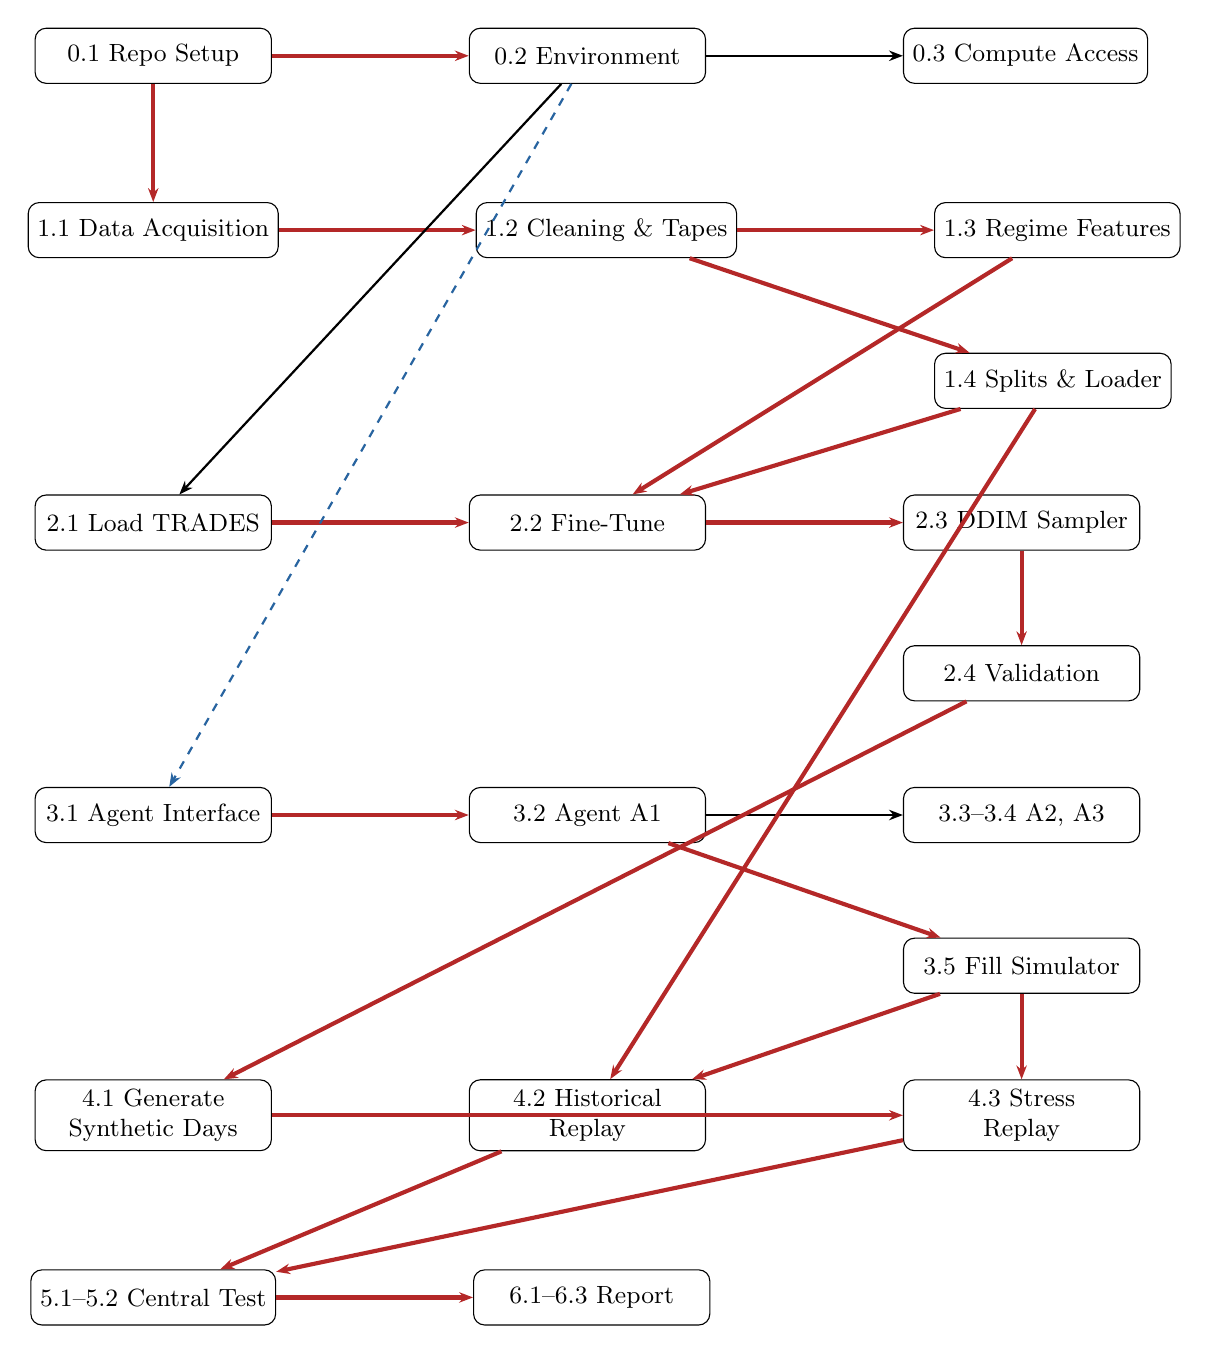
\begin{tikzpicture}[
  node distance=1.2cm and 2.5cm,
  every node/.style={draw, rounded corners, minimum width=3cm, minimum height=0.7cm, font=\small, align=center},
  arr/.style={-{Stealth[length=5pt]}, thick},
  crit/.style={arr, line width=1.5pt, color=critical},
  par/.style={arr, dashed, color=deepening}
]

% Phase 0
\node (repo) {0.1 Repo Setup};
\node (env) [right=of repo] {0.2 Environment};
\node (compute) [right=of env] {0.3 Compute Access};

% Phase 1
\node (acq) [below=1.5cm of repo] {1.1 Data Acquisition};
\node (clean) [right=of acq] {1.2 Cleaning \& Tapes};
\node (regime) [right=of clean] {1.3 Regime Features};
\node (splits) [below right=of clean] {1.4 Splits \& Loader};

% Phase 2
\node (ckpt) [below=3cm of acq] {2.1 Load TRADES};
\node (finetune) [right=of ckpt] {2.2 Fine-Tune};
\node (ddim) [right=of finetune] {2.3 DDIM Sampler};
\node (val) [below right=of finetune] {2.4 Validation};

% Phase 3 (parallel)
\node (iface) [below=3cm of ckpt] {3.1 Agent Interface};
\node (a1) [right=of iface] {3.2 Agent A1};
\node (a2a3) [right=of a1] {3.3--3.4 A2, A3};
\node (fill) [below right=of a1] {3.5 Fill Simulator};

% Phase 4
\node (synth) [below=3cm of iface] {4.1 Generate\\Synthetic Days};
\node (hist) [right=of synth] {4.2 Historical\\Replay};
\node (stress) [right=of hist] {4.3 Stress\\Replay};

% Phase 5
\node (holdout) [below=1.5cm of synth] {5.1--5.2 Central Test};

% Phase 6
\node (report) [right=of holdout] {6.1--6.3 Report};

% Arrows
\draw[crit] (repo) -- (env);
\draw[arr] (env) -- (compute);
\draw[crit] (repo) -- (acq);
\draw[crit] (acq) -- (clean);
\draw[crit] (clean) -- (regime);
\draw[crit] (clean) -- (splits);
\draw[crit] (splits) -- (finetune);
\draw[crit] (regime) -- (finetune);
\draw[arr] (env) -- (ckpt);
\draw[crit] (ckpt) -- (finetune);
\draw[crit] (finetune) -- (ddim);
\draw[crit] (ddim) -- (val);
\draw[par] (env) -- (iface);
\draw[crit] (iface) -- (a1);
\draw[arr] (a1) -- (a2a3);
\draw[crit] (a1) -- (fill);
\draw[crit] (val) -- (synth);
\draw[crit] (fill) -- (hist);
\draw[crit] (fill) -- (stress);
\draw[crit] (synth) -- (stress);
\draw[crit] (splits) -- (hist);
\draw[crit] (stress) -- (holdout);
\draw[crit] (hist) -- (holdout);
\draw[crit] (holdout) -- (report);

\end{tikzpicture}
\end{center}

\vspace{0.3cm}
\textbf{Legend:} \textcolor{critical}{\textbf{Bold solid}} = critical path. \textcolor{deepening}{\textbf{Dashed}} = can proceed in parallel.

\vspace{0.5cm}
\noindent\textbf{Key parallelism opportunities:}
\begin{itemize}[nosep]
  \item Phase 3 (agents + fill simulator) can proceed in parallel with Phase 2 (generator training), since agents are tested first on real data.
  \item Within Phase 3, A2 and A3 are incremental extensions of A1 and can be developed concurrently by different people.
  \item Report writing should begin in Phase~1 and continue throughout.
\end{itemize}

% ══════════════════════════════════════════════════════════
%  SUMMARY TABLE
% ══════════════════════════════════════════════════════════
\newpage
\section*{Effort Summary and Role Assignments}

\begin{center}
\small
\begin{longtable}{p{0.6cm}p{4.5cm}p{2.5cm}p{1.5cm}p{3.5cm}}
\toprule
\textbf{Task} & \textbf{Description} & \textbf{Owner} & \textbf{Effort} & \textbf{Key Risk} \\
\midrule
\endfirsthead
\toprule
\textbf{Task} & \textbf{Description} & \textbf{Owner} & \textbf{Effort} & \textbf{Key Risk} \\
\midrule
\endhead
0.1 & Repository setup & Everyone & 3h & None \\
0.2 & Python environment & ML + Data & 4h & TRADES compatibility \\
0.3 & Compute \& tracking & ML Lead & 4h & GPU queue delays \\
\midrule
1.1 & Data acquisition & Data Lead & 1--2d & Depth access \\
1.2 & Cleaning \& tapes & Data Lead & 3--5d & Edge cases in TAQ \\
1.3 & Regime features & Data Lead & 2--3d & VPIN correctness \\
1.4 & Splits \& loader & Data Lead & 1--2d & Schema mismatch \\
\midrule
2.1 & Load TRADES & ML Lead & 1--2d & Schema mismatch \\
2.2 & Fine-tune conditioning & ML Lead & 3--5d & GPU budget \\
2.3 & DDIM sampler & ML Lead & 1--2d & None (standard) \\
2.4 & Generator validation & Val+MM Lead & 5--7d & \textbf{Generator fails} \\
\midrule
3.1 & Agent interface & Val+MM Lead & 1d & None \\
3.2 & Agent A1 (AS) & Val+MM Lead & 2d & $\kappa$ calibration \\
3.3 & Agent A2 (OFI) & Val+MM Lead & 1d & None \\
3.4 & Agent A3 (VPIN) & Val+MM Lead & 1d & None \\
3.5 & Fill simulator & Val+MM Lead & 3--4d & Queue-position logic \\
\midrule
4.1 & Generate synthetic days & ML Lead & 3--5d & Compute overrun \\
4.2 & Historical replay & Val+MM Lead & 1--2d & None \\
4.3 & Stress replay & Val+MM Lead & 2--3d & Agents don't separate \\
4.4 & Metrics computation & Analysis Lead & 1d & None \\
\midrule
5.1 & Holdout replay & Val+MM Lead & 1d & None \\
5.2 & Rank-correlation test & Analysis Lead & 2--3d & Weak signal \\
\midrule
6.1 & Figures & Analysis Lead & 2--3d & None \\
6.2 & Written report & Analysis Lead + all & 5--7d & Time pressure \\
6.3 & Repo cleanup & Everyone & 1--2d & None \\
\bottomrule
\end{longtable}
\end{center}

\vspace{0.3cm}
\textbf{Total estimated effort:} $\sim$45--65 person-days across 4 team members over 13 weeks.

\end{document}